\documentclass[11pt,a4paper]{article}

% --- layout -----------------------------------------------------------------
\usepackage[margin=2.4cm]{geometry}
\usepackage{microtype}
\usepackage{booktabs}
\usepackage{multirow}
\usepackage{graphicx}
\usepackage{amsmath}
\usepackage{amssymb}
\usepackage{caption}
\usepackage{subcaption}
\usepackage[table]{xcolor}
\usepackage[hidelinks]{hyperref}
\usepackage{url}
\usepackage{authblk}
\usepackage{siunitx}
\sisetup{detect-all, table-number-alignment = center}

% --- CJK (mixed-script examples appear throughout) ---------------------------
\usepackage{fontspec}
\usepackage{xeCJK}
\setCJKmainfont{Noto Serif CJK JP}
\setCJKsansfont{Noto Sans CJK JP}

\captionsetup{font=small, labelfont=bf}
\captionsetup[table]{skip=4pt}
\renewcommand{\arraystretch}{1.15}

% Author-facing marker for gaps that must be closed before submission.
\newcommand{\todo}[1]{\textcolor{red}{\textbf{[TODO: #1]}}}
\newcommand{\best}[1]{\textbf{#1}}
\newcommand{\na}{\textendash}

% ---------------------------------------------------------------------------
\title{\bfseries Synthetic Speech Overstates Code-Switching ASR:\\
A Japanese--English Reality Check with Whisper and an On-Device Audio LM}

\author[1]{Awshesh Nath Sharma}
\author[2]{Syed Ali Abbas Rahil}
\affil[1]{\normalsize University of Liverpool}
\affil[2]{\normalsize Otsuka Shokai}
\date{}

\begin{document}
\maketitle

\begin{abstract}
\noindent
Text-to-speech (TTS) synthesis is the standard workaround for the scarcity of
labelled code-switching speech, but the cost of that substitution is rarely
measured. We quantify it for Japanese--English. We fine-tune Whisper large-v3
with LoRA on a 350-clip synthetic corpus built from neural TTS and reach
\SI{2.48}{\percent} code-switching WER on its matched held-out split --- a number
that reads like a solved task. We then evaluate \emph{that same merged
checkpoint}, unchanged, on CS-FLEURS JA--EN read speech, where real human voices
read code-switched sentences. It scores \SI{36.3}{\percent} mixed error rate
(MER) and still renders \SI{27}{\percent} of English reference words outside
Latin script. The adaptation does transfer --- it improves on zero-shot Whisper
large-v3 (\SI{40.9}{\percent} MER, \SI{64.6}{\percent} script accuracy) --- but
the in-domain figure overstates deployable performance by a wide margin, and the
relative error reduction collapses from \SI{97.8}{\percent} in-domain to
\SI{11.2}{\percent} on real speech. Motivated by this gap, we adapt a second
architecture: LFM2.5-Audio-1.5B-JP, a hybrid state-space/attention audio language
model with a Conformer encoder. Applying LoRA to the \emph{acoustic encoder}
rather than the decoder alone lifts script accuracy from \SI{37.4}{\percent} to
\SI{80.8}{\percent} and cuts MER to \SI{27.0}{\percent} on the same frozen
benchmark, surpassing both Whisper systems on code-switching while leaving
Japanese monolingual accuracy intact (CER \SI{6.6}{\percent} $\rightarrow$
\SI{6.4}{\percent}). English monolingual recognition remains the outstanding
weakness (\SI{37.1}{\percent} WER against Whisper's \SI{4.2}{\percent}). We argue
that script fidelity, not word error rate, is the metric that exposes
synthetic-to-real degradation, and that encoder-side adaptation --- not decoder
prompting or decoder-only LoRA --- is what actually buys code-switching capability.
\end{abstract}

\medskip
\noindent\textbf{Keywords:} code-switching, speech recognition, low-resource
adaptation, LoRA, synthetic training data, Japanese

% ===========================================================================
\section{Introduction}
% ===========================================================================

Code-switching --- alternating between two languages within a single utterance
--- is routine in Japanese professional speech, where English technical
vocabulary is embedded in Japanese syntactic frames. A speaker asks
\mbox{「次のmeetingはいつ？」} (``When is the next meeting?'') without pausing at
the language boundary. Automatic speech recognition systems trained on
monolingual corpora handle this poorly: they collapse output to one language,
force English words into katakana, or drop the minority language entirely. The
failure is not merely cosmetic. Downstream tasks --- action-item extraction,
search, summarisation --- operate on the transcript, and a transcript that renders
\emph{deadline} as \mbox{デッドライン} has silently destroyed the string an
enterprise pipeline was looking for.

The binding constraint on progress is data. Labelled, naturally-occurring
code-switched speech is expensive to elicit and annotate, and for Japanese--English
it is essentially unavailable at scale --- a scarcity that has left the pair far
behind Mandarin--English, where the SEAME corpus~\cite{lyu2010seame} has supported
a decade of work. The field's standard response is to synthesise: draft
code-switched sentences with a language model, render them with neural TTS, and
fine-tune on the result. The approach is fast, cheap, perfectly aligned by
construction, and increasingly common. What it costs in generalisation is
almost never measured, because the same synthetic distribution supplies both the
training and the test split.

This paper measures that cost. Our design is deliberately simple: train on
synthetic speech, then evaluate the resulting checkpoint on real speech without
touching it. We report both numbers for the same model, and the difference
between them is the paper's primary result.

Measuring the gap requires the right instrument. Word error rate is a poor one
here, because the dominant code-switching failure --- rendering an English word
in katakana instead of Latin script --- is scored as a single substitution,
indistinguishable from any ordinary misrecognition. We therefore adopt
\emph{script accuracy}: the fraction of English reference words that the system
renders in Latin script rather than katakana, another script, or not at all. It
isolates the code-switching behaviour from general recognition quality, and it
turns out to be the metric on which synthetic training and real speech diverge
most sharply.

Our contributions are:
\begin{enumerate}
  \itemsep2pt
  \item \textbf{A quantified synthetic-to-real gap for code-switching ASR.} A
    Whisper large-v3 LoRA checkpoint that achieves \SI{2.48}{\percent} CS-WER on
    its matched synthetic test split retains only \SI{11.2}{\percent} relative MER
    improvement over zero-shot on real code-switched read speech, against
    \SI{97.8}{\percent} in-domain (Section~\ref{sec:gap}).
  \item \textbf{Evidence that encoder adaptation, not decoder adaptation, drives
    code-switching gains.} On LFM2.5-Audio, decoder-side LoRA with data
    augmentation moves script accuracy by \SI{6.2}{} points; adding LoRA to the
    Conformer encoder adds a further \SI{18.2}{} points
    (Section~\ref{sec:results}).
  \item \textbf{A frozen, reusable JA--EN evaluation protocol} combining a
    code-switched test set with matched monolingual controls drawn from the same
    sentences and speakers, so that forgetting is separable from domain shift
    (Section~\ref{sec:eval}).
  \item \textbf{A deployable on-device result}: \SI{80.8}{\percent} script
    accuracy from a 1.5\,B-parameter model with
    8.16\,M trainable parameters, running faster than real time
    on an \SI{8}{\giga\byte} laptop GPU (Section~\ref{sec:deployment}).
\end{enumerate}

We also report a negative result plainly: our best code-switching model remains
far behind Whisper on English monolingual audio (\SI{37.1}{\percent} versus
\SI{4.2}{\percent} WER). We consider this the most important open problem the
work leaves behind, and we do not discount it.

% ===========================================================================
\section{Background and Related Work}
% ===========================================================================

\subsection{Multilingual and code-switching ASR}

End-to-end architectures displaced HMM-GMM pipelines~\cite{rabiner1989} through
CTC~\cite{graves2006ctc}, attention-based encoder-decoders~\cite{chan2015las},
and the Conformer~\cite{gulati2020conformer}, whose interleaving of self-attention
with convolution remains the dominant audio encoder design.
Whisper~\cite{radford2022whisper} trained an encoder-decoder Transformer on
680\,k hours of weakly supervised audio across 96 languages,
producing a model whose multilingual prior is strong enough that adaptation to a
new task often requires hundreds rather than thousands of hours. Massively
multilingual efforts~\cite{pratap2020mls,zhang2023usm} extended the same scaling
argument further.

Code-switching has been studied linguistically for
decades~\cite{poplack1980,myersscotton1993}. The Matrix Language Frame
model~\cite{myersscotton1993} holds that one language supplies the morphosyntactic
frame while the other contributes content morphemes; in Japanese--English
discourse Japanese is consistently the matrix language, with English nouns and
technical terms inserted at positions Japanese syntax permits. This asymmetry
matters for ASR: English lexical items occur in acoustic contexts shaped by
Japanese prosody and co-articulation, distributions a monolingual English model
has never observed.

Computational work has concentrated on Mandarin--English, where
SEAME~\cite{lyu2010seame} provides real conversational data. Shan et
al.~\cite{shan2019cs} added language-aware attention; Winata et
al.~\cite{winata2020meta} applied meta-transfer learning for few-shot adaptation.
Both required either large labelled code-switching corpora or expensive
meta-training. Peng et al.~\cite{peng2023prompting} showed that Whisper's
pre-training is strong enough that prompting alone recovers substantial
code-switching ability, reducing the in-domain data requirement by orders of
magnitude. Japanese--English has received comparatively little attention, and
CS-FLEURS~\cite{yan2025csfleurs} is the first broad-coverage benchmark to include
the pair.

\subsection{Parameter-efficient fine-tuning}

LoRA~\cite{hu2021lora} reparameterises a weight update as a low-rank product
$\Delta W = BA$ with $B \in \mathbb{R}^{m \times r}$, $A \in \mathbb{R}^{r \times
n}$ and $r \ll \min(m,n)$, freezing $W$ and training only $A$ and $B$. Because
$B$ is zero-initialised, $\Delta W = 0$ at the start of training and the adapted
model begins from the full strength of the pre-trained weights --- a property that
matters when the adaptation set is small enough that a random perturbation would
be destructive. Alternatives include adapter
modules~\cite{houlsby2019adapters}, prefix tuning~\cite{li2021prefix}, and prompt
tuning~\cite{lester2021prompt}; LoRA is preferred here because the adapter can be
merged into the base weights after training, incurring no inference-time
overhead. Aghajanyan et al.~\cite{aghajanyan2020intrinsic} give the theoretical
motivation: fine-tuning updates occupy a subspace whose effective dimension is far
below the ambient one, and scales with task complexity and dataset size.

\subsection{Synthetic speech as training data}

Using TTS to manufacture training audio is well established for low-resource ASR,
and augmentation with recorded noise~\cite{snyder2015musan},
spectrogram masking~\cite{park2019specaugment}, and speed
perturbation~\cite{ko2015audio} are standard complements. For code-switching
specifically, synthesis is unusually attractive: a language model can generate
switch points on demand, and the resulting transcript is exact by construction,
eliminating the inter-annotator disagreement that plagues manual code-switching
annotation~\cite{yilmaz2018semi}. CS-FLEURS~\cite{yan2025csfleurs} itself uses
synthesis for the majority of its test sets, reserving real voices for a
14-language subset.

The literature is correspondingly thin on what synthesis costs. Y{\i}lmaz et
al.~\cite{yilmaz2018semi} compared augmentation strategies for code-switching but
did not isolate synthetic-versus-real training audio. To our knowledge, no prior
work evaluates a single code-switching checkpoint on both a matched synthetic
test set and real speech, which is precisely the comparison we report.

% ===========================================================================
\section{Corpora}
\label{sec:corpora}
% ===========================================================================

\subsection{The synthetic training corpus}

The training corpus contains 350 clips: 100 code-switching, 200 Japanese-only,
and 50 English-only. Source sentences were drafted with a large language model
and rendered with Microsoft Azure neural TTS --- \texttt{en-US-JennyNeural} for
English units and a \texttt{ja-JP} female neural voice for Japanese --- at
\SI{24}{\kilo\hertz} mono. Code-switching clips concatenate per-unit renderings in
language-alternation order with approximately \SI{1.2}{\second} of silence at each
junction; monolingual clips use \SI{300}{\milli\second}. Because each clip is
rendered \emph{from} its transcript, audio and reference are exactly aligned and
annotation noise is zero.

A 70/30 utterance-level split with a fixed seed gives 245 training and 105 test
clips (Table~\ref{tab:corpus}). Training audio is augmented with
MUSAN~\cite{snyder2015musan} noise at \SI{20}{\deci\bel} and \SI{15}{\deci\bel}
SNR, giving $2 \times 245$ augmented variants plus the originals for 735 training
samples.

\begin{table}[t]
\centering
\caption{Synthetic corpus composition. The 70/30 split is utterance-level with a
fixed seed; augmentation applies to the training partition only.}
\label{tab:corpus}
\small
\begin{tabular}{lrrrr}
\toprule
Category & Train & Test & Total & Augmented train \\
\midrule
Code-switching  &  70 &  30 & 100 & 210 \\
Japanese-only   & 140 &  60 & 200 & 420 \\
English-only    &  35 &  15 &  50 & 105 \\
\midrule
Total           & 245 & 105 & 350 & 735 \\
\bottomrule
\end{tabular}
\end{table}

Two properties of this corpus are essential to the argument. First, it is
\emph{convenient}: it was assembled in days, at negligible cost, with perfect
labels. Second, it is \emph{narrow}: one voice per language, no disfluencies, no
prosodic switch cues, no channel variability, and inter-unit silences that are a
synthesis artefact rather than a property of bilingual speech. These are exactly
the properties a practitioner accepts when choosing synthesis, and exactly the
ones whose cost we set out to measure.

\subsection{The real-speech evaluation benchmark}

Evaluation uses CS-FLEURS~\cite{yan2025csfleurs}, built over
FLEURS~\cite{conneau2023fleurs}. We take the entire Japanese--English
\texttt{read/test} slice: 196 utterances in which \emph{human speakers read
code-switched sentences}. The sentences are constructed by aligning FLEURS
translations and swapping spans, so the switch points are synthetic; the acoustics
are not. This is the axis on which our training corpus is weakest, and therefore
the axis worth testing.

Critically, no CS-FLEURS data of any split is used in training. The training
corpus is generated independently, so the full 196-utterance slice is a clean
held-out set and the same fixed utterances score every system in this paper.

\subsection{Monolingual controls}

We add two 200-utterance monolingual sets from FLEURS \texttt{ja\_jp} and
\texttt{en\_us} test. Because CS-FLEURS is constructed by span-swapping over the
\emph{same} FLEURS sentences, in the same style and register, these controls are
matched rather than merely adjacent: a monolingual regression after fine-tuning is
attributable to the adaptation, not to a domain shift between benchmarks. This
lets us separate ``learned to code-switch'' from ``forgot how to do Japanese''.

% ===========================================================================
\section{Evaluation Methodology}
\label{sec:eval}
% ===========================================================================

\subsection{Metrics}

Mixed-script transcription defeats naive word-level scoring, because Japanese has
no orthographic word boundaries. We therefore score four quantities, each over an
explicitly defined token stream, with identical normalisation (NFKC, lowercasing,
punctuation mapped to space, English fillers removed) applied to references and to
every hypothesis.

\textbf{Script accuracy (ScriptAcc)} is the headline. Of the English words in the
reference, it is the fraction the system renders in Latin script:
\begin{equation}
\mathrm{ScriptAcc} = \frac{\left|\{\, w \in R_{\mathrm{en}} : \hat{w} \text{ is Latin-script} \,\}\right|}{|R_{\mathrm{en}}|}
\end{equation}
where $R_{\mathrm{en}}$ is the set of English reference words. A word forced into
katakana, rendered in another script, or dropped all count against it. ScriptAcc
answers the question a bilingual user actually asks --- \emph{did it keep my
English as English?} --- and, unlike WER, it is unaffected by ordinary
recognition errors elsewhere in the utterance.

\textbf{Mixed error rate (MER)} is an edit rate over a mixed token stream, taking
one token per Japanese character and one per English word, which avoids dependence
on a Japanese word segmenter. \textbf{JA-CER} is character error rate over the
Japanese-only stream and \textbf{JA-WER} its word-level counterpart via
\texttt{fugashi} segmentation; \textbf{EN-WER} is word error rate over the Latin
stream. The monolingual metrics are forgetting controls, not headline results.

\subsection{A note on metric commensurability}
\label{sec:commensurability}

The dissertation-stage experiments on the synthetic corpus report
\textbf{CS-WER}: whitespace-delimited word error rate over the mixed reference.
The real-speech benchmark reports MER. \emph{These are different metrics, computed
over different token streams, on different test sets, and their absolute values
must not be subtracted or divided across the two settings.} We are explicit about
this because the temptation to write ``\num{2.48}\,\% became \num{36.3}\,\%, a
\num{15}$\times$ degradation'' is strong and the statement would be unsound.

What \emph{is} sound is a comparison of each system against a common baseline
\emph{within} each setting. On the synthetic set, LoRA reduces CS-WER from
\SI{111.57}{\percent} (zero-shot) to \SI{2.48}{\percent}, a \SI{97.8}{\percent}
relative reduction. On real speech, the same checkpoint reduces MER from
\SI{40.9}{\percent} (zero-shot) to \SI{36.3}{\percent}, a \SI{11.2}{\percent}
relative reduction. Both are relative improvements over the same base model, each
measured with one metric on one set, and it is their \emph{ratio of relative
gains} --- not the raw error rates --- that quantifies how much of the adaptation
survives contact with real speech.

\subsection{Inference protocol}

Every system is evaluated under one protocol. LFM systems use the system prompt
\texttt{"Perform ASR."}, matching their training data; the base model is strongly
prompt-sensitive, so this is held fixed across conditions. Whisper systems run
through \texttt{transformers} on GPU with automatic language detection,
\texttt{repetition\_penalty}\,$=1.3$ and \texttt{no\_repeat\_ngram\_size}\,$=3$ to
suppress the decoding loops both models exhibit on code-switched input. Metrics
are pooled corpus-wide rather than averaged per utterance, avoiding the
instability short utterances introduce.

% ===========================================================================
\section{Whisper LoRA Adaptation}
\label{sec:whisper}
% ===========================================================================

We adapt Whisper large-v3 (1.5\,B parameters, 32-layer encoder
and decoder, $d_{\text{model}}=1280$, 128-mel front end) with LoRA on the query and
value projections of the decoder attention layers, freezing the encoder entirely.
The configuration is $r=8$, $\alpha=16$, dropout \num{0.1}, learning rate
\num{1e-4} held constant, effective batch size 16 (4 per device $\times$ 4
accumulation steps), bf16 precision. This yields roughly 3.9\,M
trainable parameters, \SI{0.26}{\percent} of the base model.

Freezing the encoder encodes a hypothesis: that Whisper's multilingual
pre-training already supplies adequate acoustic representations for both
languages, and that code-switching adaptation is principally a matter of adjusting
the decoder's language prior. Section~\ref{sec:lfm} tests that hypothesis
directly, and finds it wanting.

Two implementation details proved decisive. Japanese language forcing via
\texttt{forced\_decoder\_ids} must be applied at inference; without it the
untrained decoder emits predominantly English for code-switched audio, since
English dominates Whisper's pre-training distribution. And label padding positions
must be masked to $-100$ so that cross-entropy ignores them --- with the leading
BOS token stripped, since the trainer prepends it during teacher forcing.

Development proceeded in four phases. Phase~1 established Small and Medium
baselines. Phase~2 was invalidated by a data-loading defect that read an empty
column, yielding empty references and meaningless error rates; we report it here
because the failure is instructive and because its checkpoints must not be
mistaken for results. Phase~3 fixed the defect and compared three large-v3
configurations (Table~\ref{tab:phase3}). Phase~4 extended the winner to 15 epochs,
warm-started from the Phase~3 checkpoint.

\begin{table}[t]
\centering
\caption{Phase~3 configuration comparison on the synthetic test split. Learning
rate dominates rank: both \num{5e-5} runs fail to converge within the budget.}
\label{tab:phase3}
\small
\begin{tabular}{llrlrr}
\toprule
Configuration & LR & $r$ & Modules & Best ep. & CS-WER (\%) \\
\midrule
\texttt{v3\_r8\_1e4}     & \num{1e-4} & 8 & q, v            & 8 & \best{6.61} \\
\texttt{v3\_r4\_5e5}     & \num{5e-5} & 4 & q, v            & 7 & 85.95 \\
\texttt{v3\_r8\_attn4}   & \num{5e-5} & 8 & q, v, k, out    & 8 & 45.45 \\
\bottomrule
\end{tabular}
\end{table}

The final checkpoint is merged into the base weights and published as a
standalone model, which is the artefact evaluated on real speech in
Section~\ref{sec:gap}. No further training of any kind is applied to it.

% ===========================================================================
\section{LFM2.5-Audio Adaptation}
\label{sec:lfm}
% ===========================================================================

The synthetic-to-real result motivated a second system built on a different
inductive bias. LFM2.5-Audio-1.5B-JP~\cite{liquidai2025lfm2audio} pairs a hybrid
state-space/attention language backbone with a 17-layer Conformer audio encoder
and an MLP adapter, at 1.5\,B parameters total. Unlike Whisper it
is designed for on-device deployment, and unlike Whisper its encoder is small
enough to adapt cheaply.

\subsection{Where to put the adapters}

The package ships no LoRA support, so adapters are attached manually via PEFT.
This freedom is the point of the experiment. We compare two placements:

\textbf{Decoder-side only.} LoRA on the language backbone --- attention
projections \texttt{q\_proj}, \texttt{k\_proj}, \texttt{v\_proj},
\texttt{out\_proj}, the state-space \texttt{in\_proj}, and feed-forward
\texttt{w1}, \texttt{w2}, \texttt{w3} --- with $r=8$, $\alpha=16$, dropout
\num{0.05}. This is the direct analogue of the Whisper recipe and yields
approximately 4.7\,M trainable parameters
(\SI{0.32}{\percent}).

\textbf{Encoder \emph{and} decoder.} The same backbone targets plus LoRA on the
Conformer's attention (\texttt{linear\_q}, \texttt{linear\_k}, \texttt{linear\_v},
\texttt{linear\_out}) and feed-forward (\texttt{linear1}, \texttt{linear2})
projections. The pointwise convolutions are \texttt{Conv1d} and are left alone.
This gives \num{8155136} trainable parameters (\SI{0.5579}{\percent}).

Encoder and backbone adapters are optimised as two AdamW parameter groups with
separate learning rates: \num{3e-5} for the backbone and \num{6e-6} --- five times
lower --- for the encoder. The asymmetry is deliberate. The encoder carries
phonological representations learned from far more audio than we can supply, and
an aggressive update destroys them; the backbone's language prior is what we
actually intend to move.

\subsection{Training data}

Training uses the synthetic corpus of Section~\ref{sec:corpora}, extended with
MUSAN augmentation at three levels (noise at \SI{20}{\deci\bel} and
\SI{13}{\deci\bel}, music at \SI{20}{\deci\bel}) and a task taxonomy that pairs
each audio type with a directed system prompt (\texttt{"Perform ASR."},
\texttt{"Perform ASR in Japanese."}, \texttt{"Perform ASR in English."}). The
best-performing run additionally mixes in FLEURS-balanced monolingual data to
counter English forgetting.

\todo{The best configuration reported in Table~\ref{tab:real} (rank-32 encoder
LoRA with the FLEURS-balanced mix) is not covered by the project training log,
which stops at the preceding run. Recover and document its step count, learning
rates, data proportions, and validation curve before submission --- the paper's
strongest number currently has no reproducible recipe.}

% ===========================================================================
\section{Results}
\label{sec:results}
% ===========================================================================

\subsection{In-domain performance on synthetic speech}

Table~\ref{tab:synthetic} reports all three Whisper scales on the matched
synthetic test split. Error rates are low across the board and fall monotonically
with model size on code-switching audio, reaching \SI{2.48}{\percent} CS-WER for
large-v3. Read in isolation, this table says the task is solved.

\begin{table}[t]
\centering
\caption{Whisper LoRA results on the \emph{synthetic} held-out split
($n=105$). RTF and VRAM are single-sample inference measurements. These numbers
are in-domain: training and test share one TTS distribution and one voice per
language.}
\label{tab:synthetic}
\small
\begin{tabular}{lrrrrrrrr}
\toprule
& & \multicolumn{3}{c}{WER (\%) $\downarrow$} & \multicolumn{3}{c}{CER (\%) $\downarrow$} & \\
\cmidrule(lr){3-5}\cmidrule(lr){6-8}
Model & Params & CS & JA & EN & CS & JA & EN & VRAM \\
\midrule
Whisper Small     & 244\,M & 9.92 & 10.00 & 1.90 & 0.99 & 1.09 & 1.01 & \SI{0.54}{\giga\byte} \\
Whisper Medium    & 769\,M & 6.61 & \best{0.00} & \best{0.32} & 0.40 & \best{0.00} & \best{0.05} & \SI{1.59}{\giga\byte} \\
Whisper large-v3  & 1.5\,B & \best{2.48} & 0.83 & 2.22 & \best{0.40} & 0.05 & 1.61 & \SI{3.13}{\giga\byte} \\
\midrule
\multicolumn{2}{l}{\emph{large-v3, zero-shot}} & 111.57 & 100.00 & 1.59 & \na & \na & \na & \na \\
\bottomrule
\end{tabular}
\end{table}

The training trajectory (Table~\ref{tab:phase4}) shows a phase structure worth
noting: Japanese WER collapses from \SI{100}{\percent} to \SI{4.2}{\percent} by
epoch~4 while CS-WER remains above \SI{70}{\percent}, and only between epochs~5
and~7 does CS-WER fall steeply. The model learns Japanese phonology first and
language switching second. Terminating on a fixed patience at epoch~5 would have
recorded this configuration as a failure.

\begin{table}[t]
\centering
\caption{Phase~4 training trajectory, \texttt{v3\_r8\_1e4} extended to 15 epochs.
Code-switching competence emerges abruptly between epochs~5 and~7, well after
Japanese monolingual accuracy has converged.}
\label{tab:phase4}
\small
\begin{tabular}{lrrrrrrrr}
\toprule
Epoch & 0 & 1 & 4 & 7 & 8 & 10 & 12 & 15 \\
\midrule
CS-WER (\%) & 111.57 & 104.96 & 71.90 & 7.44 & 5.79 & 4.96 & 4.96 & \best{2.48} \\
JA-WER (\%) & 100.00 & 100.00 & 4.17 & 3.33 & 2.50 & 0.83 & 0.83 & 0.83 \\
EN-WER (\%) & 1.59 & 1.90 & 1.90 & 1.90 & 1.90 & 1.59 & 2.22 & 2.22 \\
\bottomrule
\end{tabular}
\end{table}

\subsection{Performance on real code-switched speech}

Table~\ref{tab:real} is the paper's central table. Every system is scored on the
same frozen 196-utterance CS-FLEURS slice and the same monolingual controls.

\begin{table}[t]
\centering
\caption{Results on the frozen real-speech benchmark: CS-FLEURS JA--EN
\texttt{read/test} ($n=196$, code-switching) with matched FLEURS monolingual
controls ($n=200$ each). ScriptAcc is the headline code-switching metric; the
monolingual columns are forgetting controls. Whisper large-v3 + LoRA is the
\emph{same merged checkpoint} that scores \SI{2.48}{\percent} CS-WER in
Table~\ref{tab:synthetic}.}
\label{tab:real}
\small
\begin{tabular}{lrrrrr}
\toprule
& \multicolumn{2}{c}{Code-switching} & \multicolumn{3}{c}{Monolingual controls} \\
\cmidrule(lr){2-3}\cmidrule(lr){4-6}
System & ScriptAcc $\uparrow$ & MER $\downarrow$ & JA-CER $\downarrow$ & JA-WER $\downarrow$ & EN-WER $\downarrow$ \\
\midrule
LFM2.5-Audio-1.5B-JP (zero-shot)      & 37.4 & 67.3 & 6.6 & 7.6 & 68.5 \\
Whisper large-v3 (zero-shot)          & 64.6 & 40.9 & \best{6.0} & 7.9 & \best{4.2} \\
\midrule
\multicolumn{6}{l}{\emph{This work}} \\
Whisper large-v3 + LoRA (synthetic-trained) & 73.0 & 36.3 & \na & \na & \na \\
LFM + LoRA, augmentation only               & 43.6 & 54.3 & 8.2 & 8.7 & 80.2 \\
LFM + LoRA, {}+ Conformer encoder LoRA      & 61.8 & 54.1 & 9.4 & 10.2 & 73.1 \\
LFM + LoRA, $r{=}32$ encoder {}+ FLEURS mix & \best{80.8} & \best{27.0} & 6.4 & \best{7.2} & 37.1 \\
\bottomrule
\multicolumn{6}{l}{\footnotesize \na{} = not measured. See Section~\ref{sec:limitations}.} \\
\end{tabular}
\end{table}

Four findings follow.

\textbf{The base models disagree sharply on code-switching.} Whisper large-v3
zero-shot keeps \SI{64.6}{\percent} of English words in Latin script;
LFM2.5-Audio-1.5B-JP keeps \SI{37.4}{\percent}. The Japanese-specialised model is
markedly worse at preserving English, which is consistent with its training
emphasis and is the deficit our adaptation targets.

\textbf{Encoder LoRA is what moves script accuracy.} Decoder-side LoRA with data
augmentation raises ScriptAcc from \SI{37.4}{\percent} to \SI{43.6}{\percent}
($+6.2$). Adding LoRA to the Conformer encoder --- holding the data fixed ---
raises it to \SI{61.8}{\percent} ($+18.2$), roughly three times the gain from
decoder adaptation. This is a clean single-variable comparison and it directly
contradicts the frozen-encoder assumption underlying the Whisper recipe in
Section~\ref{sec:whisper}. \emph{We note that the final row changes two things at
once} --- rank $8 \rightarrow 32$ and the addition of the FLEURS-balanced mix ---
so its $+19.0$ further gain cannot be attributed to either factor alone.

\textbf{Code-switching gains need not cost Japanese.} The best configuration ends
at JA-CER \SI{6.4}{\percent} against the base model's \SI{6.6}{\percent} and
JA-WER \SI{7.2}{\percent} against \SI{7.6}{\percent} --- marginally better, not
worse. Because the monolingual controls are drawn from the same sentences and
speakers as the code-switching set, this is evidence of genuinely retained
capability rather than an artefact of benchmark mismatch. The intermediate rows
show the mechanism is not automatic: the two weaker configurations both degrade
Japanese (to \SI{8.2}{\percent} and \SI{9.4}{\percent} CER) before the balanced
data mix restores it.

\textbf{English monolingual recognition is the unresolved failure.} Every LFM
configuration is far behind Whisper on English-only audio. The base model starts
at \SI{68.5}{\percent} EN-WER; decoder-only LoRA makes it \emph{worse}
(\SI{80.2}{\percent}); the best configuration recovers to \SI{37.1}{\percent},
roughly half the base error but nearly nine times Whisper's \SI{4.2}{\percent}. A
system that keeps English in Latin script but transcribes English audio at
\SI{37}{\percent} WER is useful for bilingual meetings and unsuitable as a general
English recogniser. We state this plainly rather than confining it to a limitations
paragraph.

\begin{figure}[t]
\centering
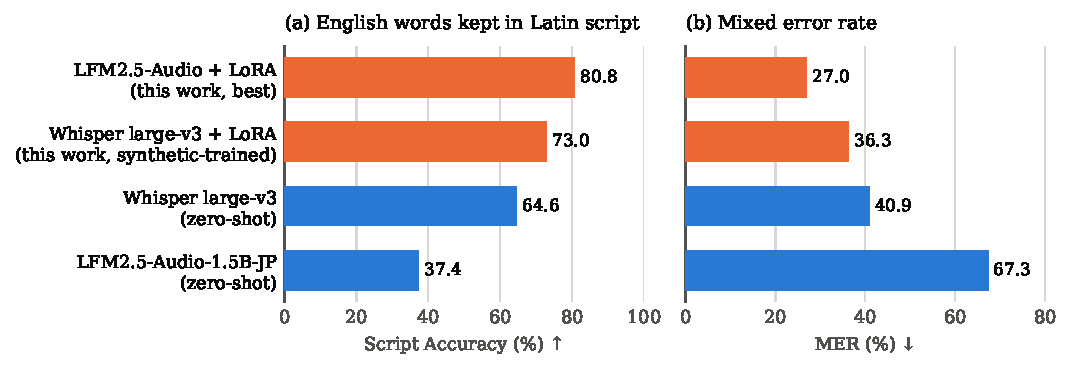
\includegraphics[width=\textwidth]{figures/fig_real_benchmark.pdf}
\caption{Systems on the frozen real-speech benchmark (CS-FLEURS JA--EN,
$n=196$). ScriptAcc and MER differ in scale and direction and are therefore
plotted on separate axes, never shared. Orange marks systems from this work.}
\label{fig:benchmark}
\end{figure}

\subsection{Ablations on the synthetic corpus}

The ablations below were run on Whisper Small for tractability and are reported
for what they are: evidence about \emph{the synthetic training regime}, not about
real-speech performance. They are informative for practitioners building similar
corpora and should not be read as generalising to natural speech.

\begin{table}[t]
\centering
\caption{Ablations on the synthetic corpus (Whisper Small). Each varies one factor
with all others held fixed. Note the scale: without augmentation the model does
not learn the task at all.}
\label{tab:ablations}
\small
\begin{tabular}{lrrrr}
\toprule
Condition & CS-WER (\%) & CS-CER (\%) & JA-WER (\%) & EN-WER (\%) \\
\midrule
\multicolumn{5}{l}{\emph{(a) Noise augmentation level}} \\
\quad None                        & 271.90 & 55.71 & 33.33 & 2.54 \\
\quad SNR \SI{20}{\deci\bel}      & 171.90 & 23.17 & 21.67 & 2.86 \\
\quad SNR 20{+}15                 &  17.36 &  2.38 & 15.83 & 2.22 \\
\quad SNR 20{+}15{+}10{+}5        & \best{13.22} & \best{1.06} & \best{11.67} & \best{1.90} \\
\midrule
\multicolumn{5}{l}{\emph{(b) LoRA rank (q, v projections)}} \\
\quad $r=4$                       & 55.37 & 4.88 & 24.17 & 2.86 \\
\quad $r=8$                       & 16.53 & 2.64 & 21.67 & 2.22 \\
\quad $r=16$                      & \best{14.05} & \best{2.24} & 17.50 & 2.22 \\
\quad $r=32$                      & 18.18 & 2.24 & \best{14.17} & \best{1.90} \\
\midrule
\multicolumn{5}{l}{\emph{(c) Training data composition}} \\
\quad CS only                     & 255.37 & 56.77 & 95.83 & 4.13 \\
\quad JA only                     & 682.64 & 172.34 & 27.50 & 2.86 \\
\quad CS {+} JA                   &  23.97 & \best{2.97} & \best{15.83} & \best{1.90} \\
\quad CS {+} JA {+} EN            & \best{17.36} & 2.51 & 17.50 & 2.86 \\
\bottomrule
\end{tabular}
\end{table}

Three observations. \emph{Noise augmentation is not optional}: without it CS-WER
sits at the untrained baseline, and the second SNR level produces a tenfold
improvement --- a threshold effect, not a gradual one. \emph{Rank is non-monotonic}:
$r=16$ is optimal for Small, with $r=32$ degrading through overfitting on 70
code-switching training clips, consistent with the intrinsic-dimensionality
account of Aghajanyan et al.~\cite{aghajanyan2020intrinsic}. \emph{Monolingual
data is necessary}: training on code-switching audio alone leaves CS-WER at the
untrained baseline, and adding English-only clips improves code-switching
performance despite contributing only 35 training utterances. For corpus
builders, the practical implication is that monolingual recordings --- cheap, and
available from existing corpora~\cite{sonobe2017jsut,panayotov2015librispeech} ---
carry disproportionate value relative to expensive code-switched elicitation.

% ===========================================================================
\section{The Synthetic-to-Real Gap}
\label{sec:gap}
% ===========================================================================

We now compare the two settings for a single checkpoint. The model is Whisper
large-v3 with the $r{=}8$, \num{1e-4}, 15-epoch adapter merged into the base
weights. It is evaluated on its matched synthetic test split and on CS-FLEURS
JA--EN with no intervening training, no recalibration, and no prompt changes
beyond the shared protocol of Section~\ref{sec:eval}.

Following Section~\ref{sec:commensurability}, we compare relative improvements
over the same zero-shot base model within each setting:
\begin{center}
\begin{tabular}{lrrr}
\toprule
Setting & Zero-shot & + LoRA & Relative gain \\
\midrule
Synthetic TTS test split ($n=105$), CS-WER & 111.57 & 2.48 & \SI{97.8}{\percent} \\
CS-FLEURS JA--EN ($n=196$), MER            &  40.90 & 36.30 & \SI{11.2}{\percent} \\
\bottomrule
\end{tabular}
\end{center}

\begin{figure}[t]
\centering
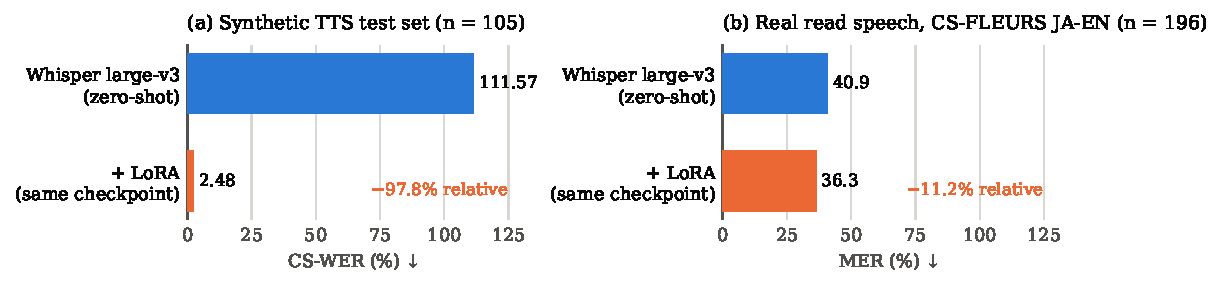
\includegraphics[width=\textwidth]{figures/fig_gap.pdf}
\caption{The same merged checkpoint on two test sets. Each panel has its own
metric and axis --- CS-WER and MER are not commensurable
(Section~\ref{sec:commensurability}) --- so the comparison is between the
\emph{relative} gains over a shared zero-shot baseline, not between raw values.}
\label{fig:gap}
\end{figure}

The adaptation transfers, but weakly. Nearly all of the in-domain improvement is
attributable to fitting the synthetic distribution rather than to acquiring
code-switching capability that survives a change of speaker and channel. On
ScriptAcc the picture is the same: the fine-tuned checkpoint reaches
\SI{73.0}{\percent} against zero-shot Whisper's \SI{64.6}{\percent}, an
\num{8.4}-point gain, and it still fails to preserve Latin script for more than a
quarter of English reference words.

Why the degradation is this large follows from Section~\ref{sec:corpora}. The
training corpus has one voice per language, so the model may minimise loss by
keying on voice-specific spectral regularities rather than on language-general
acoustics. It has fixed inter-unit silences at switch points, so the model can
learn to treat silence as a switch cue --- a cue that does not exist in the fluent
switches of CS-FLEURS. It has no disfluencies, no prosodic switch marking, and no
channel variation. None of these are exotic failure modes; they are the direct,
predictable consequences of the corpus design, and the size of the gap is our
estimate of what they cost.

We draw two conclusions for practice. First, \textbf{a synthetic held-out split is
not a validation set for a synthetically-trained code-switching model}; it
measures fit to the synthesiser. Any claim about deployable performance needs
real speech, even a small quantity of it. Second, \textbf{script accuracy exposes
the gap better than word error rate}. It moves \num{8.4} points where relative MER
gain collapses from \SI{97.8}{\percent} to \SI{11.2}{\percent}, and it names the
specific failure --- katakana substitution --- that makes a transcript unusable
downstream while barely registering as a WER penalty.

% ===========================================================================
\section{Deployment}
\label{sec:deployment}
% ===========================================================================

The motivating application is on-device transcription of privacy-sensitive
bilingual meetings, where sending audio to a cloud API is prohibited. We
therefore measure inference on consumer hardware: an NVIDIA RTX 4060 Laptop GPU
(\SI{8}{\giga\byte} VRAM, Ada Lovelace) in a Dell G15, with merged checkpoints
loaded from local disk, one warm-up pass, fp16 for Small and Medium and bf16 for
large-v3.

\begin{table}[t]
\centering
\caption{Inference on an RTX 4060 Laptop GPU (\SI{8}{\giga\byte}), averaged over
six clips (mean duration \SI{11.1}{\second}). RTF is inference time divided by
audio duration; all three models run far below real time and fit concurrently in
\SI{8}{\giga\byte}.}
\label{tab:deployment}
\small
\begin{tabular}{lrrrrr}
\toprule
Model & Params & Precision & Model VRAM & Mean inference & Mean RTF \\
\midrule
Whisper Small    & 244\,M & fp16 & \SI{478}{\mega\byte}  & \SI{0.192}{\second} & 0.020 \\
Whisper Medium   & 769\,M & fp16 & \SI{1458}{\mega\byte} & \SI{0.445}{\second} & 0.048 \\
Whisper large-v3 & 1.5\,B & bf16 & \SI{2945}{\mega\byte} & \SI{0.651}{\second} & 0.064 \\
\bottomrule
\end{tabular}
\end{table}

All three models run one to two orders of magnitude faster than real time, and all
three load simultaneously in roughly \SI{4.9}{\giga\byte} --- meaning a
side-by-side comparison interface fits on a mid-range laptop. Latency, not
throughput, would bind in a live-captioning deployment.

Two generation artefacts appeared during benchmarking and are worth recording,
since aggregate error rates conceal them. Whisper large-v3 entered a repetition
loop on one code-switching clip (\texttt{何かadviceadad\ldots}), and Whisper
Medium hallucinated a Japanese transcript for English-only audio. Both are known
autoregressive failure modes, both are mitigated by the repetition penalty and
$n$-gram blocking in our evaluation protocol, and both indicate that a deployed
system needs decoding safeguards independent of its error rate on a benchmark.

% ===========================================================================
\section{Limitations}
\label{sec:limitations}
% ===========================================================================

\textbf{The real-speech benchmark is small and single-speaker.} CS-FLEURS
JA--EN \texttt{read/test} contains 196 utterances from one speaker. Results are
therefore speaker-specific, and we report no confidence intervals; bootstrap
resampling over utterances is the obvious remedy and has not been run.
Additionally, CS-FLEURS switch points are generated by span-swapping, making them
denser and more regular than natural conversational switching, so absolute error
rates on it run high relative to what naturalistic speech would produce.

\textbf{One incomplete row.} The Whisper large-v3 + LoRA system has not been
scored on the FLEURS monolingual controls, so its forgetting profile is unknown
and Table~\ref{tab:real} carries three empty cells. The evaluation harness
supports this directly; the run has simply not been performed.

\textbf{One undocumented recipe.} As flagged in Section~\ref{sec:lfm}, the
training configuration for the best-performing LFM row is not recorded in the
project logs. Until recovered, that row is a measurement without a method.

\textbf{Confounded final ablation step.} The transition from \SI{61.8}{\percent}
to \SI{80.8}{\percent} ScriptAcc changes LoRA rank and training data
simultaneously. The individual contributions are not separable from the runs
performed.

\textbf{No seed variance.} Every configuration was trained once. Reported
differences below roughly two points should not be treated as reliable
orderings.

\textbf{Synthetic-corpus ablations do not transfer automatically.} The
augmentation, rank, and composition results in Table~\ref{tab:ablations} were
measured in the synthetic regime, and the central finding of this paper is
precisely that conclusions drawn there need not hold on real speech.

% ===========================================================================
\section{Conclusion}
% ===========================================================================

We set out to measure what synthetic training data costs in code-switching ASR,
and found the cost to be large. A Whisper large-v3 LoRA checkpoint that reduces
code-switching error by \SI{97.8}{\percent} relative on its matched synthetic test
split retains only \SI{11.2}{\percent} relative improvement when the same
checkpoint meets real code-switched read speech. The adaptation is genuine but
modest; the in-domain number is mostly a measurement of fit to the synthesiser.
Practitioners should treat a synthetic held-out split as a training diagnostic
rather than as evidence of deployability, and should adopt script accuracy
alongside word error rate, because it names the failure --- English forced into
katakana --- that ruins a transcript downstream while barely moving WER.

The constructive half of the paper is that architecture placement matters more
than we expected. Adapting the Conformer encoder of LFM2.5-Audio, rather than the
language backbone alone, produced roughly three times the script-accuracy gain of
decoder-side adaptation, and the best configuration reached \SI{80.8}{\percent}
ScriptAcc and \SI{27.0}{\percent} MER --- surpassing Whisper large-v3 on
code-switching --- while leaving Japanese monolingual accuracy intact and running
faster than real time on an \SI{8}{\giga\byte} laptop GPU. The frozen-encoder
convention inherited from text-domain LoRA practice appears to be the wrong
default when the task is acoustic language alternation rather than a shift in
output style.

What remains open is English. Our best code-switching system transcribes
English-only audio at \SI{37.1}{\percent} WER against Whisper's
\SI{4.2}{\percent}, and closing that gap without surrendering script accuracy is
the natural next problem. Beyond it, the priorities that follow from this work are
a speaker-diverse real-speech evaluation set with confidence intervals, the
separation of rank from data mixture in the final ablation, and a direct test of
whether encoder-side adaptation confers the same advantage on Whisper that it
does on LFM2.5-Audio.

% ===========================================================================
\section*{Reproducibility}

Training, preprocessing, and evaluation code, the scoring harness with unit tests,
and the CS-FLEURS and FLEURS loaders are available in the project repository. The
merged Whisper checkpoint evaluated in Section~\ref{sec:gap} and the LFM adapters
are published on the Hugging Face Hub. Raw prediction files from the real-speech
evaluation are not currently version-controlled; the numbers in
Table~\ref{tab:real} are transcribed from project evaluation logs, and
regenerating them from the published checkpoints is a documented single-command
operation.

\bibliographystyle{plain}
\bibliography{refs}

\end{document}
